\documentclass[
  dvipdfmx
]{standalone}
\usepackage{tikz}
\usetikzlibrary{spath3}
\usetikzlibrary{knots}
\usetikzlibrary{hobby}
\usetikzlibrary{patterns}
\begin{document}
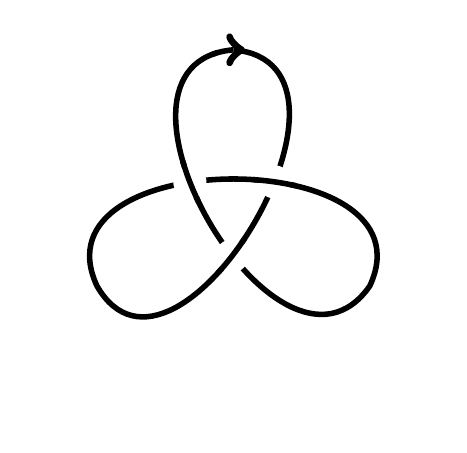
\begin{tikzpicture}
    \begin{knot}[
      consider self intersections=true,
      ignore endpoint intersections=false,
      % draft mode=crossings,
      every strand/.append style={line width=2pt},
      flip crossing=3,
      clip width=10,
      clip radius=6pt,
      % background color=red,
    ]
    \strand (0,2)
    .. controls +(5:-2) and +(235:2) .. (-30:2)
    .. controls +(65:2) and +(115:2) .. (210:2)
    .. controls +(300:2) and +(-5:2) .. (0,2);
    \end{knot}
    % \strand[draw=black, line width=2pt] (210:2)
    % .. controls +(300:2) and +(-5:2) .. (0,2);
    \draw[->, line width=3pt] (0.05,2) -- ++(0.1,0);
    % \fill[black] (0.5,0.33) circle[radius=5pt];
  \end{tikzpicture}
\end{document}